\section{Cardinal spline 3D}

Для начала поговорим о Cardinal spline 3D. Это один из видов гладких кривых, строится изначально по массиву точек $p_k$, а также $m_k$, что является тангенсом наклона кривой при прохождении данной точки. Для каждых двух точек из заданного массива имеем апроксимацию:

$$
p(t) = (2t^3 - 3t^2 + 1)p_k + (t^3 - 2t^2 + t)(x_{k+1} - x_k)m_k + 
$$
$$
+ (-2t^3 + 3t^2)p_{k+1} + (t^3 - t^2)(x_{k+1} - x_k)m_{k+1}
$$

где $x_k$ для $k = 1, ... , n$ - интеполяционная сетка, $t \in [0,1]$, а

$$
m_k = \dfrac{p_{k+1} - p_k}{2(t_{k+1} - t_k)} + \dfrac{p_{k} - p_{k-1}}{2(t_{k} - t_{k-1})}
$$

или

$$
m_k = (1-c) \dfrac{p_{k+1} - p_{k-1}}{t_{k+1} - t_{k-1}}
$$

$c \in [0,1)$, при $c=0$ называется сплайном Катмалла-Рома. 

Но в данной работе для вычисления $m_k$ я использовал функции Kochanek-Bartels Spline, выглядят они примерно так:

$$
d_i = \dfrac{(1-t)(1+b)(1+c)}{2} (p_i - p_{i-1}) + \dfrac{(1-t)(1-b)(1-c)}{2} (p_{i+1} - p_i)
$$

$$
d_{i+1} = \dfrac{(1-t)(1+b)(1-c)}{2} (p_{i+1} - p_{i}) + \dfrac{(1-t)(1-b)(1+c)}{2} (p_{i+2} - p_{i+1})
$$

где $t$ - регулирует длину вектора тангенса, $b$ - направление вектора тангенса, $c$ - так называемый continuity, задающий остроту угла между векторами. Далее пример:


\includegraphics[scale=0.45]{pictures/4.png}


\section{Кинематическая поверхность}

Сам способ задания такого рода поверхности состоит из двух составляющих: направляющая, а также сама фигура.

С направляющей разобрались, она задается пользователем по точкам, далее интерполируется, достраивается до определенной точности, чтобы казаться достаточно гладкой.

Далее стоит разобраться с видами, есть кинематические повехности переноса, они перемещают образующую фигуру по направлению направляющей кривой. Также существует вариант также с каждым переносом образующей, поворачивать ее вдволь тангенса наклона направляющей, к примеру поместив круг в основание, перемещая и вращая образующую мы получим фигуру трубы постоянного радиуса.

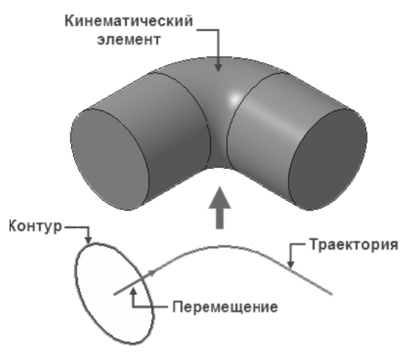
\includegraphics[scale=0.5]{pictures/1.jpg}

Так как мне не сказано какой вид поверхности строить, долго пытаясь реализовать полноценный поворот образующей, я остановился на первом варианте.

\begin{lstlisting}[language=Javascript]
var a = res_dots[i];
var b = res_dots[i+1];
var step = 30;
for (var fi = 0; fi <= 360; fi += step) {
    var x_1 = cos(fi / 360 * 2 * PI) * document.getElementById('a').value;
    var z_1 = sin(fi / 360 * 2 * PI) * document.getElementById('b').value;
    var x_2 = cos((fi + step) / 360 * 2 * PI) * document.getElementById('a').value;
    var z_2 = sin((fi + step) / 360 * 2 * PI) * document.getElementById('b').value;
    beginShape();
    vertex(x_1 + a.x, a.y, z_1 + a.z);
    vertex(x_2 + a.x, a.y, z_2 + a.z);
    vertex(x_2 + a.x + piv.x, a.y + piv.y, z_2 + a.z + piv.z);
    vertex(x_1 + a.x + piv.x, a.y + piv.y, z_1 + a.z + piv.z);
    endShape(CLOSE);
}
\end{lstlisting}

Данный фрагмент кода отрисовывает одну боковую грань цилиндра для каждых двух точек направляющей кривой. Точность регулируется переменной $step$.

\begin{lstlisting}[language=Javascript]
// demo
control_points = [
    {x:-400,y:400,z:0},
    {x:-200,y:-400,z:0},
    {x:200,y:100,z:0},
    {x:400,y:-200,z:0}
];
\end{lstlisting}

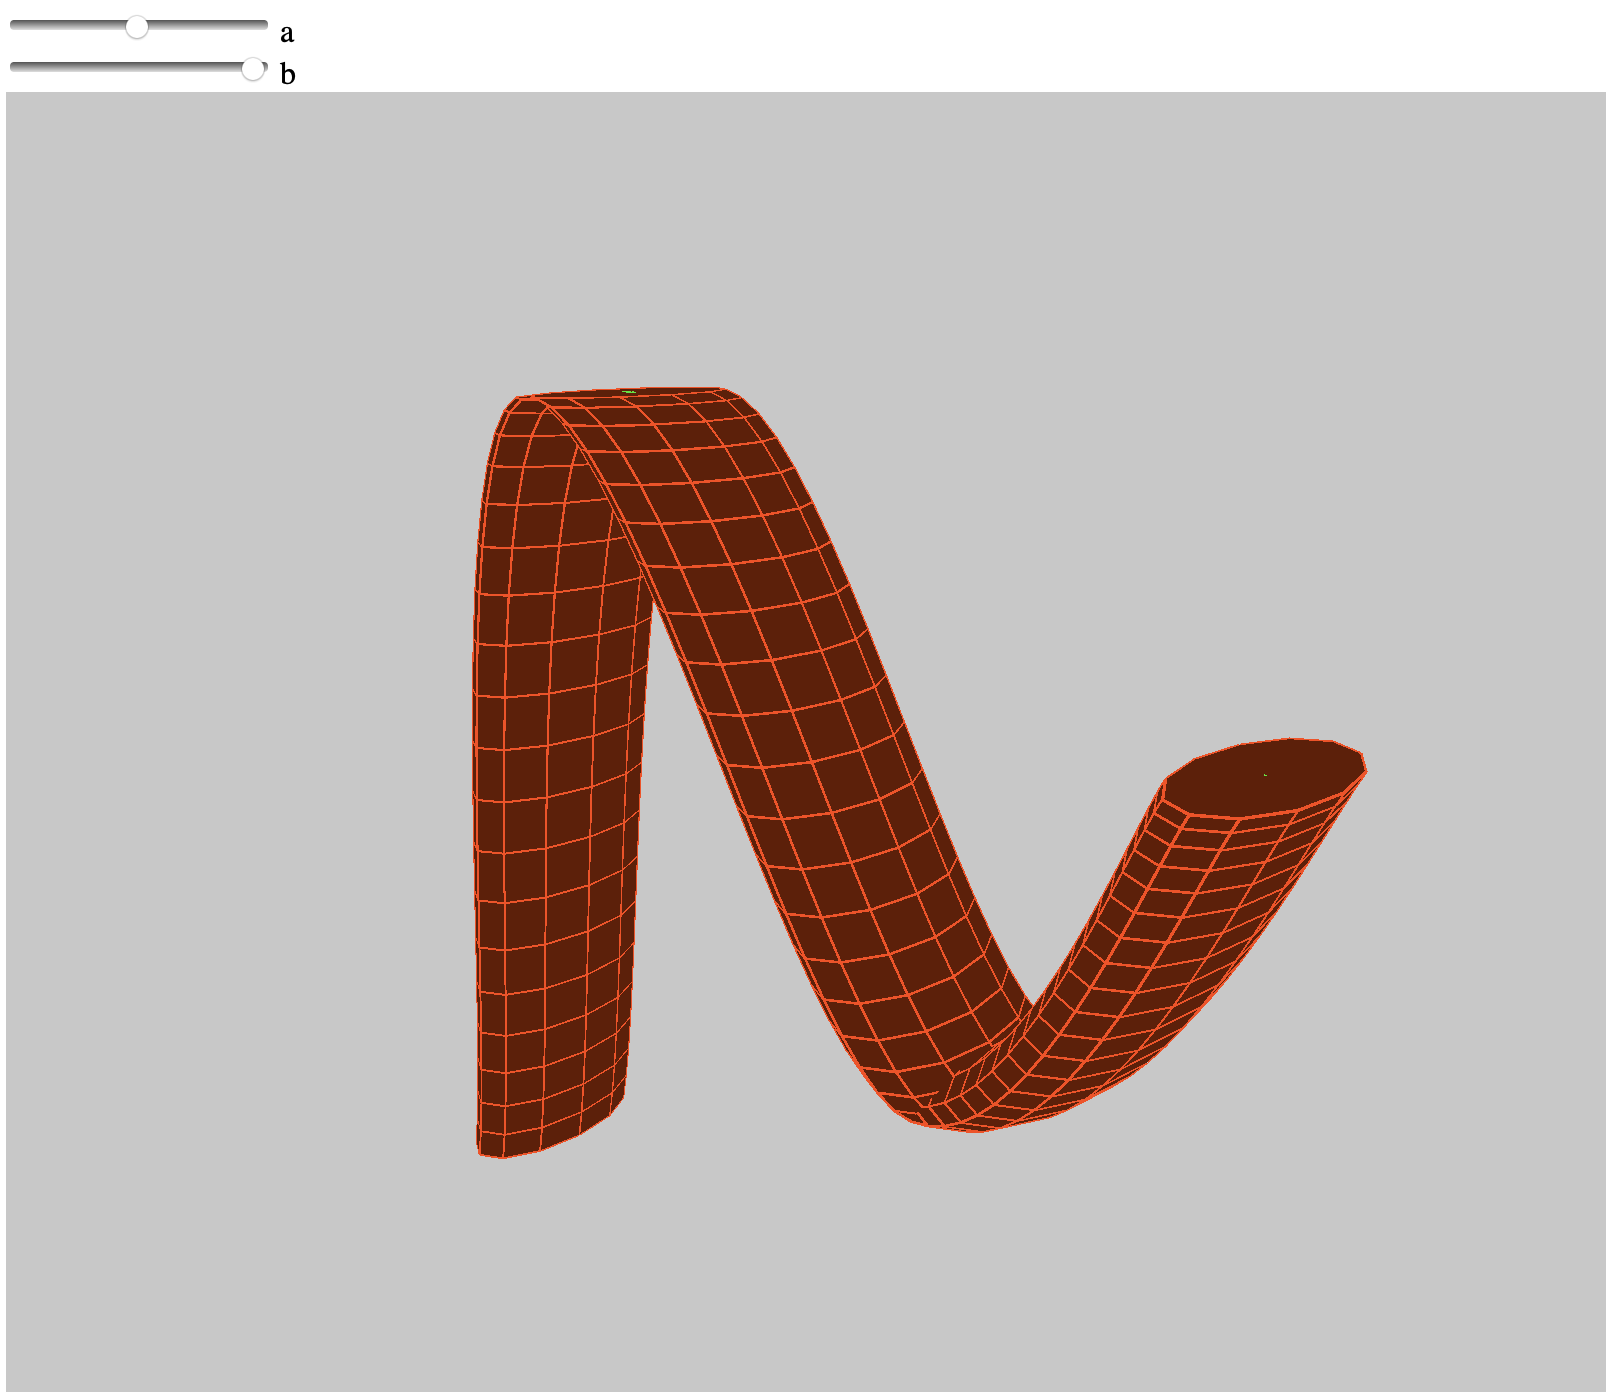
\includegraphics[scale=0.35]{pictures/2.png}

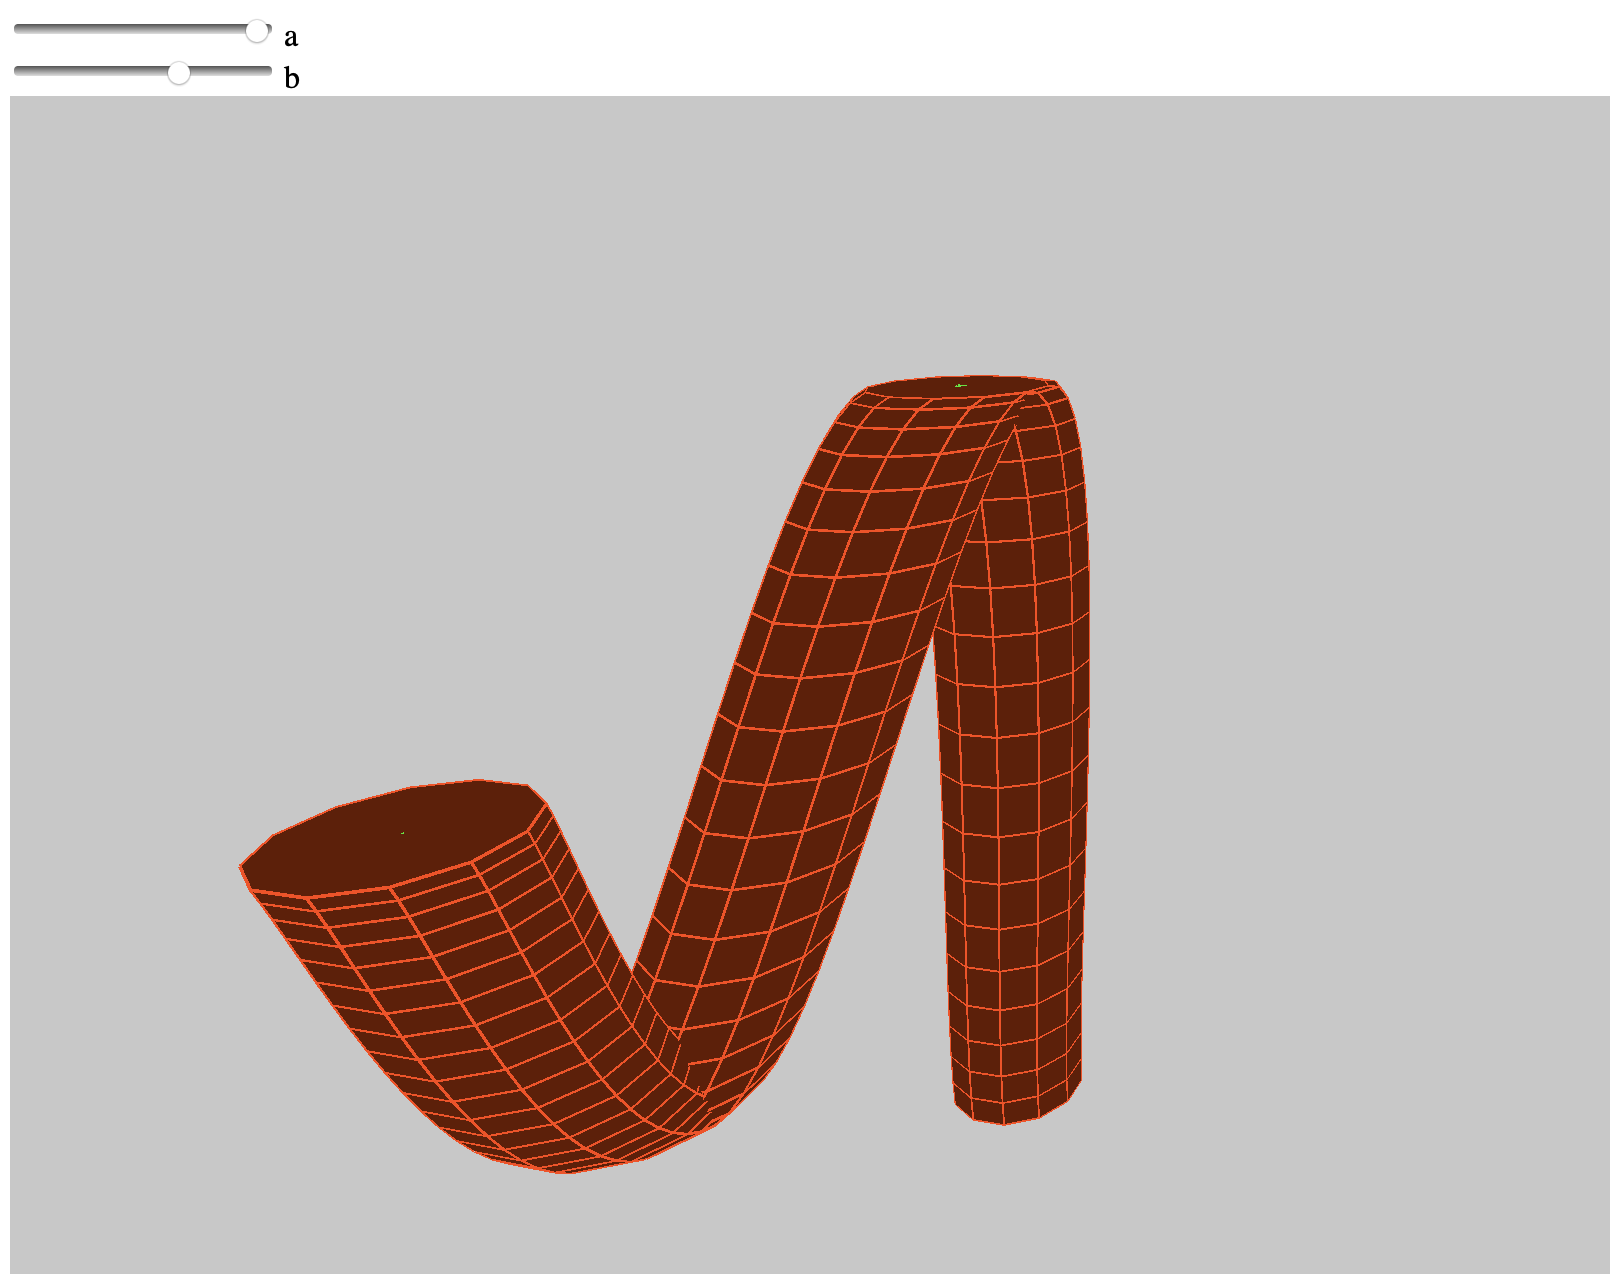
\includegraphics[scale=0.35]{pictures/3.png}

\begin{lstlisting}[language=Javascript]
//heart
control_points = [
    {x:0,y:400,z:-300},
    {x:-400,y:0,z:-200},
    {x:-200,y:-400,z:-100},
    {x:0,y:-200,z:0},
    {x:200,y:-400,z:100},
    {x:400,y:0,z:200},
    {x:0,y:400,z:300}
];
\end{lstlisting}

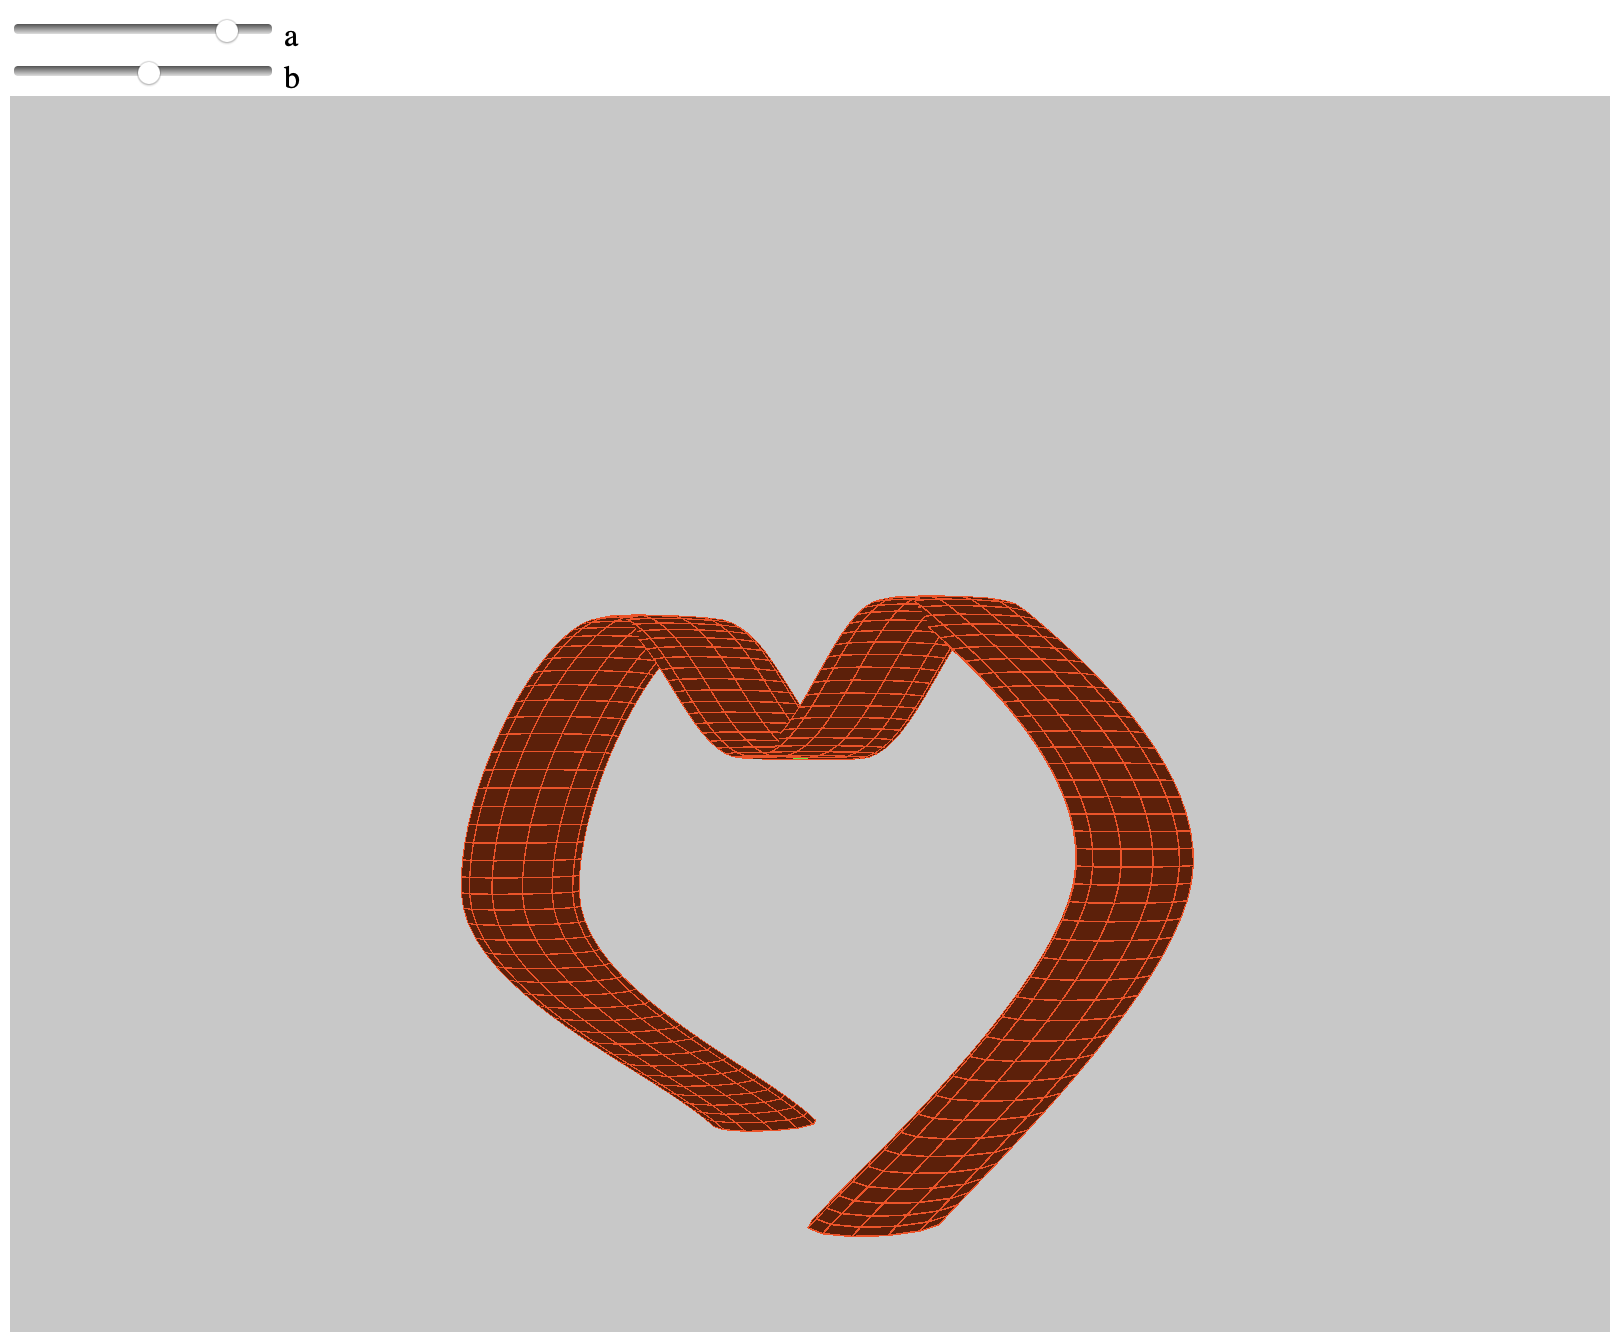
\includegraphics[scale=0.35]{pictures/5.png}